%! TeX program = lualatex
\documentclass[../main.tex]{subfiles}
\begin{document} \section{Recursive models}

Does geometric intuition always lead to the right choice of model?

\begin{example} \label{ex:intro-population}
  Our intern found some bacteria living in a petri dish and checked in every hour to find the following data. They created a log-log plot and suggested the model \(P = 100 t^{2}\). 

  \begin{minipage}{0.65\textwidth}
    \centering
    \begin{tabular}{r|r|l}
      time \(t\)  & observed population \(P\) & intern's model \(P = 100 t^{2}\) \\ \midrule
      1 & 100     & \\ \midrule
      2 & 200     & \\ \midrule
      3 & 400     & \\ \midrule
      4 & 800     & \\ \midrule
      5 & 1600    & \\ \midrule
      6 & 3200    & \\ \midrule
      7 & unknown &  
    \end{tabular}
  \end{minipage}
  \begin{minipage}{0.3\textwidth}
    \centering
    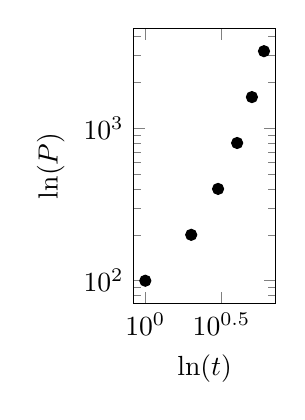
\begin{tikzpicture}
      \begin{loglogaxis}[height=2in, axis equal image, xlabel={\(\ln(t)\)}, ylabel={\(\ln(P)\)}]
        \addplot[only marks] coordinates {
            (1, 100) (2, 200) (3, 400) (4, 800) (5, 1600) (6, 3200)
          };
      \end{loglogaxis}
    \end{tikzpicture}
  \end{minipage}

  \faComment{} What is the population at \(t = 7\) predicted by our intern's model? Does this prediction make sense biologically?
  \blanklines{5}

  The above data exhibits certain pattern consistent with biological theory. Propose a description for \hlmain{such a pattern} in plain English.

  \includegraphics[page=1]{../build/polls.pdf}

  \todo{Collect some public opinion and do an iClicker poll using student provided opinions. We hope that some student shouts ``\(P\) doubles every hour!''}
\end{example}
\clearpage

Example~\ref{ex:intro-population} suggests that some natural phenomena can be described by an earlier version of itself. 

\begin{mdframed}[style=simple-compact]
 A \hlmain{recursive model} describes data in terms of one or more earlier versions of itself.
\end{mdframed}

\begin{example}
  Let \(w_{t}\) denote the weight (grams) of a radioactive material at time \(t\) (years). Therefore, \(w_{0}\) is its current weight. 

  Such material loses half of its weight every years. 
  \begin{enumerate}[wide]
    \item Suppose \(w_{0} = 200\). What is its weight in \(3\) years?
      \blanklines{10}
    \item Let \(t \ge 1\) be a variable. Write down a mathematical expression for \(w_{t}\) in terms of \(w_{t-1}\).
      \blanklines{10}
    \item Let \(t \ge 1\) be a variable. Write down a mathematical expression for \(w_{t}\) as a function of \(t\) and \(w_{0}\).
      \blanklines{10}
  \end{enumerate}

  What did we just do? 
  \begin{itemize}[itemsep=2ex]
    \item In part 2, we gave a \underline{\hspace{2in}} description of \(w_{1}, w_{2}, w_{3}, \ldots\). 
    \item In part 3, we gave a \underline{\hspace{2in}} description of \(w_{1}, w_{2}, w_{3}, \ldots\). 
  \end{itemize}
\end{example}

\clearpage

\end{document}
